\chapter{LLMalMorph 的详细设计}

\section{A. LLMalMorph 框架}

在本节中,我们将详细阐述我们框架的架构(见图\ref{fig:4.1})。LLMalMorph 分为两个主要模块。第一个模块,功能变异模块使用 LLM 和策略性生成的提示来转换恶意软件源代码函数。第二个模块,变种合成模块将转换后的函数集成回源代码,编译修改后的项目以生成恶意软件变体。该模块还融入了人在回路流程用于编译期间的调试。第一个模块又包含三个关键子模块:Extractor、Prompt Generator 和 LLM Based Function Modifier。第二个模块包含两个主要子模块:Merger 以及 Compilation and Debugging。我们现在介绍支撑该框架的形式化算法,随后对各模块进行详细解释。

\begin{figure}[htbp]
	\centering
	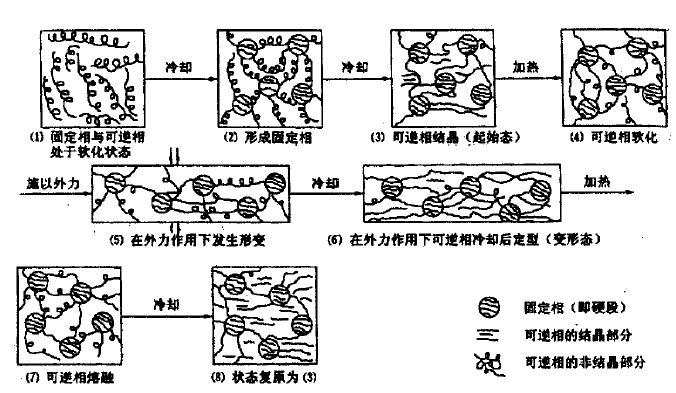
\includegraphics[width=0.75\textwidth]{figures/figure1.png}
	% \caption[这里的文字将会显示在 listoffigure 中]{这里的文字将会显示在正文中}
	\caption{LLMalMorph整体架构。该框架由两大核心模块构成:功能变异模块:从恶意软件源代码文件中提取功能函数,并借助LLM进行修改。变种合成模块:将修改后的函数更新至恶意软件源代码,通过编译项目生成变种文件}\label{fig:4.1}
\end{figure}

Algorithm \ref{alg:Function Transformation Using LLM},专为功能变异模块设计,详细说明了三个子模块 Extractor、Prompt Generator 和 LLM-Based Function Modifier 如何转换恶意软件源代码中的函数。该算法以文件名 $i$、要修改的函数数量 $j$、期望的转换策略 $s$ 以及选定的 $LLM$ 作为输入。接下来,我们将详细描述每个子模块。

\begin{algorithm}[htbp]
	\caption{使用LLM转换函数\label{alg:Function Transformation Using LLM}}
	\KwIn{文件名$i$,需要改变的函数数量 $j$,转换策略 $s$,语言模型 $LLM$}
	\KwOut{转换后的函数集$\hat{F_{s}}=\{\hat{f_{1}^{i}},\hat{f_{2}^{i}}...,\hat{f_{j}^{i}}\}$}

    Headers,globals,functions$\{f_{1}^{i},f_{2}^{i},...,f_{G}^{i}\}\leftarrow extractor(i)$;\\
    初始化转换后的函数集 $\hat{F_{s}}\leftarrow \emptyset$;\\

    \For{$t \gets 1$ \KwTo $j$}{
        $p_{s}||f_{t}^{i} \leftarrow gen\_prompt(s,f_{t}^{i},headers,globals)$;\\
        Transform function: $\hat{f_{t}^{i}} \leftarrow LLM(p_{s}||f_{t}^{i})$;\\
        Update set: $\hat{F_{s}} \leftarrow \hat{F_{s}} \cup \{\hat{f_{t}^{i}}\}$;
    }
    return $\hat{F_{s}}$
\end{algorithm}

\subsection{Extractor子模块}
Extractor 子模块(算法 \ref{alg:Function Transformation Using LLM} 的第 1 行)利用 extractor 子程序,该子程序接收一个源文件并遍历源代码的解析树。它从解析树中提取并存储以下两条辅助信息:全局声明的变量、结构体、编译器指令的列表,并将它们存储于 $globals$ 中;以及所包含头文件的列表,并将它们存储于 $headers$ 中。此类信息对于成功转换至关重要,因为它提供了函数可能使用的全局依赖项的基本上下文。以提示的形式将此上下文提供给 LLM 可确保生成更准确且语法正确的代码。此后,该子程序解析源文件以提取所有函数定义,生成集合$\{f_{1}^{i},f_{2}^{i},...,f_{G}^{i}\}$。

\subsection{Prompt Generator子模块}
算法 \ref{alg:Function Transformation Using LLM} 的第 3−7 行对应于 Prompt Generator 和 LLM Transformation 子模块。第 4 行中的子程序 $gen\_prompt$ 被调用,参数为函数 $f_t^{i}$、转换策略 $s$ 以及提取的 $headers$ 和 $globals$。它将输入代码和策略构造成一个为 LLM 定制的提示 $p_{s}||f_{t}^{i}$。提示的设计详见第 IV-C 节。另请参阅附录 F 了解该子程序中使用的不同类型的提示,以及附录 G 了解一个完整构建的提示及其相应 LLM 响应的示例。

\subsection{LLM Based Function Modifier子模块}
算法 \ref{alg:Function Transformation Using LLM}的第5行将设计好的提示 $p_{s}||f_{t}^{i}$ 提供给选定的$LLM$,并获取转换后的函数。在代码生成过程中,我们使用了LLM的默认推理设置。具体而言,temperature=0.8,top-k=40,top-p=0.9。我们在附录A-A中提供了使用LLM进行代码生成过程的详细描述。

最后,第 6 行将转换后的函数 $f_{t}^{i}$ 追加到输出集合中。一旦所有选定的函数处理完毕,该算法即返回转换后的集合。我们注意到,该算法可以执行多次,以从同一源文件生成函数的多个变体。然而,在本工作中,对于每个选定的恶意软件样本,我们将评估限制在转换后函数的单一版本上。

Algorithm \ref{alg:Malware Variant Generation},在变种合成模块中实现,使用由算法 \ref{alg:Function Transformation Using LLM} 产生的转换后函数集合 $\hat{F_{s}}$、恶意软件项目 $P$ 以及被修改的文件 $i$。它以增量方式生成恶意软件变体,并结合手动调试以确保成功编译。第 1 行初始化恶意软件变体的结果集合 $M_{s}$。该集合包含针对文件 $i$ 使用策略 $s$ 生成的恶意软件变体。尽管我们展示了针对某个特定文件的算法,但当我们处理后续文件时,先前处理过的文件的所有修改都会被保留并向前传递,从而确保恶意软件代码库的累积式转换。该算法的核心功能封装在第 2-10 行中,其中每个转换后的函数被迭代地集成和调试。

\begin{algorithm}[htbp]
	\caption{恶意软件变种生成\label{alg:Malware Variant Generation}}
	\KwIn{恶意软件项目$P$,文件名 $i$,转换后的函数集合 $\{\hat{f_{1}^{i}},\hat{f_{2}^{i}}...,\hat{f_{j}^{i}}\}$}
	\KwOut{编译后的恶意软件变种集合$M_{s}$}
    初始化集合: $M_s \leftarrow \emptyset$;\\
    \For{$t \gets 1$ \KwTo $j$}{
        Extract subset of functions: $\hat{F_{t}} \leftarrow \{\hat{f_{k}^{i}} \in \hat{F_{s}} | 1\leq k\leq t\}$;\\   
        Generate updated file: $\hat{i} \leftarrow merger(i,\hat{F_{t}})$;\\
        \While{$compile(P)$ fails}{
            Debug project $P$ and resolve errors;
        }
        Compile project: $\hat{M_{s}} \leftarrow compile(P)$;\\
        Add compiled malware: $M_{s} \leftarrow M_{s} \cup \hat{M_{s}}$;\\
    }
    return $M_{s}$
\end{algorithm}